\documentclass[11pt]{article}
\usepackage[utf8]{inputenc}	% Para caracteres en español
\usepackage{amsmath,amsthm,amsfonts,amssymb,amscd}
\usepackage{multirow,booktabs}
\usepackage[table]{xcolor}
\usepackage{fullpage}
\usepackage{lastpage}
\usepackage{enumitem}
\usepackage{fancyhdr}
\usepackage{mathrsfs}
\usepackage{wrapfig}
\usepackage{setspace}
\usepackage{calc}
\usepackage{multicol}
\usepackage{cancel}
\usepackage[retainorgcmds]{IEEEtrantools}
\usepackage[margin=3cm]{geometry}
\usepackage{amsmath}
\newlength{\tabcont}
\setlength{\parindent}{0.0in}
\setlength{\parskip}{0.05in}
\usepackage{empheq}
\usepackage{framed}
\usepackage[most]{tcolorbox}
\usepackage{xcolor}
\colorlet{shadecolor}{orange!15}
\parindent 0in
\parskip 12pt
\geometry{margin=1in, headsep=0.25in}
\theoremstyle{definition}
\newtheorem{defn}{Definition}
\newtheorem{reg}{Rule}
\newtheorem{exer}{Exercise}
\newtheorem{sln}{Solution}
\newtheorem{note}{Note}
\begin{document}
\setcounter{section}{0}
\title{}

\thispagestyle{empty}
\begin{center}
\textsc{\LARGE German University in Cairo}\\[1.0cm]
{\LARGE \bf Lectures 16}\\ [0.5cm]
{\large \bf Math301}\\ [0.5cm]
Fall 2020
\end{center}
\tableofcontents
\section{Lecture 6}
\begin{reg}
Fubini's Thm.
\end{reg}
says that double integrals are just iterated integrals. So you integrate wrt a variable while the other is const and then integrate again wrt too the other one.
\begin{reg}
How to solve double integrals of areas ?
\end{reg}
We have two cases I, II
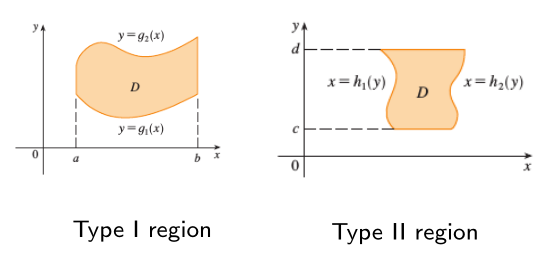
\includegraphics[scale=0.5]{images/1.png}\\ 
So how to know which region we are talking about ?
\\ simply type I as we see we draw two vertical lines making a recctangle (look at the roman I) \\
and type two is a the same rectangle but horizontal\\
So for type I regions:
\begin{equation}
	\iint \limits_D f(x,y) dA = \int_a^b [\int_{y=g_1(x)}^{y=g_2(x) }f(x,y) dy] dx 
\end{equation}
and for type II regions:
\begin{equation}
	\iint \limits_D f(x,y) dA = \int_c^d [\int_{x=u_1(x)}^{x=u_2(x) }f(x,y) dx] dy 
\end{equation}
\begin{reg}
Where to use double integrals ?
\end{reg}
\begin{enumerate}

\item Volume Calculation 
	\\ from the double integral defention it's so clear that it's used to calculate volumes :)
\begin{align}
	Volume = Area * hight \\
	V = \iint \limits_D f(x,y) dA \\
	\text{we assume the function to be our hight (z-coordinate)}
\end{align}
\item Area Calculation
	\\ if we thought of $f(x,y)=1$ then the integral is just an area
	\begin{equation}
	V = \iint \limits_D 1 dA = A
\end{equation}

\item Mass computation \\
	if we thought of $f(x,y) =\rho(x,y) $
	\\ $Total Mass = mass density * total area$
	\begin{equation}
		Mass = \iint \limits_D \rho(x,y) dA 
	\end{equation}
	
\item Charge computation \\
	if we thought of $f(x,y) =\sigma(x,y) $
	\\ $Total Charge= mass density * total area$
	\begin{equation}
		Charge = \iint \limits_D \sigma(x,y) dA 
	\end{equation}
\item moment of inertia
\item center of gravity of flat regions 
\item etc. you can find more in the textbook Stewart's Section 15.5
\end{enumerate}
\end{document}
